\documentclass{ieeeaccess}
\usepackage{cite}
\usepackage{amsmath,amssymb,amsfonts}
\usepackage{algorithmic}
\usepackage{graphicx}
\usepackage{textcomp}
\usepackage{multirow}
\makeindex

\def\BibTeX{{\rm B\kern-.05em{\sc i\kern-.025em b}\kern-.08em
    T\kern-.1667em\lower.7ex\hbox{E}\kern-.125emX}}
\begin{document}
\history{Date of publication June 20, 2019, date of current version June 20, 2019.}
\doi{}

\title{Methods to Overcome the Real-World Deep Learning Application Problems}
\author{
	\uppercase{Sangheon Lee}\authorrefmark{1}, \IEEEmembership{Student Member, IEEE},
	\uppercase{Yusung Kim}\authorrefmark{2}, \IEEEmembership{Member, IEEE}, and
	\uppercase{Jee-Hyong Lee}\authorrefmark{3}, \IEEEmembership{Fellow, IEEE}}
	
\address[1]{Department of Electrical and Computer Engineering, Sungkyunkwan University, Suwon 16419, Korea (e-mail: lawlee1@skku.edu)}
\address[2]{Memory Business, Samsung Electronics, Hwaseong 18448, Korea (e-mail: yusunge.kim@samsung.com)}
\address[3]{Department of Software, Sungkyunkwan University, Suwon 16419, Korea (e-mail: john@skku.edu)}

\tfootnote{}

\markboth
{Lee \headeretal: Methods to Overcome the Real-World Deep Learning Application Problems}
{Lee \headeretal: Methods to Overcome the Real-World Deep Learning Application Problems}

\corresp{Corresponding author: Jee-Hyong Lee (e-mail: john@skku.edu).}

\begin{abstract}
In recent years, the development of machine learning, especially deep learning, and its applications have been actively studied.
Although deep learning is applied in many areas, there are still problems to be solved in order to introduce deep learning models into real-world systems.
In this paper, we summarized the papers that overcome various problems in the real-world application of the deep learning model.
For the image classification model, an adversarial attack has been proposed which causes malfunction of the model by mixing noise that is hardly distinguishable by human into the input image of the model.
As a result, the reliability of the deep learning model has been raised, and a study has been proposed to prevent the adversarial attack.
Lee \textit{et al.} proposed an adversarial detection method based on gaussian process regression using intermediate features extracted from the classification model.
The proposed detector showed higher detection performance than other detection methods when extremely few adversarial examples are used in training.
Lee \textit{et al.} proposed a deep learning model that recognizes string CAPTCHAs that widely used in internet sites.
The proposed method eliminates the noise in the CAPTCHA image through image processing, separates string image into single character images, and recognizes CAPTCHA characters by training CNN model.
As a result of experiment on CAPTCHA used in Korea ticket reservation site, the proposed model showed a high recognition rate of 85\% based on CAPTCHA.
Won \textit{et al.} proposed a deep learning model that predicts movie audience demand before opening by using a nonlinear regression model.
In addition to features provided by the KOFIC, which provides cinema information, they define features that can be used for prediction and proposed a Bi-LSTM deep learning model to perform sentimental analysis on movie reviews.
Experimental results showed that the proposed method had higher performance than other sentimental analysis methods and effectively predicted the demand of movie audience.
Won \textit{et al.} proposed a technique for effectively handling the OOV words that are not in the existing vocabulary during word embedding. 
The proposed method is a Bi-LSTM structured deep learning model named Context-Char, which embeds the OOV words using contextual and morphosyntactic information.
As a result of experiments using datasets containing the OOV words, the proposed method showed higher performance than other methods of handling OOV words.
Lim \textit{et al.} proposed an effective under-sampling technique for processing imbalanced data. 
They proposed deep representation models that extract the structural features of major class data and minor class data and calculated the degree of conformity of the data to determine under-sampling.
In the experiments using various imbalanced data, the proposed method showed higher performance than other processing methods for most datasets.

\end{abstract}

\begin{keywords}
Deep Learning, Real-World Application, Adversarial Detection, CAPTCHA, Sentimental Analysis, Out-Of-Vocabulary Words, Imbalanced Data
\end{keywords}

\titlepgskip=-15pt

\maketitle

\clearpage
\section{Detect Adversarial Example Using Gaussian Process-based Detector}
\label{first}
\subsection{Paper main theme}
Adversarial attack is a technique that causes a malfunction of the deep learning model by mixing noise that cannot be distinguished by the human into the input of the model. 
Figure \ref{fig1} at right shows an image in which the adversarial attack is applied to the image at left recognized as “panda” by the image classification model. 
The two images are not distinguished by the human eye, but the image classification model recognizes the right image as “gibbon”, rather than “panda”. 
If a deep learning model is applied to a major part of the system, the adversarial attack can lead to serious problems in system security.

Several techniques have been proposed to prevent the adversarial attack, but few defense methods that can effectively defend against various and powerful attacks have yet been proposed. 
Therefore, adversarial detection has been proposed instead of an adversarial defense, which determine whether the input of a model is an adversarial example or not. 
Many of the adversarial detection methods showed high performance against most attacks. 
However, many of the detection methods already proposed are the deep neural network-structured model, which requires a large number of adversarial examples to train.

\subsection{Proposed idea}
Lee \textit{et al.} proposed an efficient detection method for adversarial example, which is shown in figure \ref{fig2} \cite{paper1}.
The proposed method consists of two steps. First, the intermediate feature values generated by the classification model are extracted for a given image. 
The intermediate feature is the output of the last hidden layer of the classification model, indicating the classification probability for a given input. 
The classification probability of most adversarial examples is characterized by the fact that the two classes have similar values to each other, so the detector grasps these patterns and performs adversarial detection.

Second, the intermediate feature information is used to determine whether the image is an adversarial example by applying Gaussian process regression. 
Gaussian process regression is a method to infer the mean and variance of the whole data range based on the observed data, by defining the relationship between the data using the characteristics of the data.
Assuming $f(x)\sim N(0,K(\theta,x,x'))$ for the function $f(x)$ of $x$, the log marginal likelihood is as follows:

\Figure[t]()[width=0.45\textwidth]{fig1.png}
   {An adversarial image that has imperceptible perturbation added to the natural image.\label{fig1}}

\begin{equation}
	\begin{split}
		\log p(f(x)|\theta,x) = &-{\frac{1}{2}}f(x)^{T}K(\theta,x,x')^{-1}f(x) \\
		&-{\frac{1}{2}}\log{\det(K(\theta,x,x'))} \\
		&-{\frac{|x|}{2}}\log{2\pi}
	\end{split}
\end{equation}

where, $K(\theta,x,x')$ is a covariance matrix for all possible observed data pairs $(x,x')$, calculated from a pre-defined kernel function, and $\theta$ is a hyperparameter of the covariance function. 
Based on the $\theta$ that maximizes this marginal likelihood, the distribution of the function value $f(x^\ast)$ for the unobserved data $x^\ast$ is $p(y^\ast|x^\ast,f(x),x)=N(y^\ast|A,B)$. 
That is, the posterior distribution has mean function $A$ and variance function $B$, where $A$ and $B$ are calculated through the following equations:

\begin{align}
	A = & K(\theta,x^\ast,x)K(\theta,x,x')^{-1}f(x) \\
	\begin{split}
		B = & K(\theta,x^\ast,x^\ast) \\
		&-K(\theta,x^\ast,x)K(\theta,x,x')^{-1}K(\theta,x^\ast,x)^{T}
	\end{split}
\end{align}

where, $K(\theta,x^\ast,x)$ denotes the covariance values between all observed data $x$ and the new data $x^\ast$ based on the hyperparameter value $\theta$, and $K(\theta,x^\ast,x^\ast)$ is the variance value at $x^\ast$. 

In the Gaussian process regression, the influence between two data is defined as covariance. If the dimension of data is high, it is difficult to grasp the pattern of covariance between data. 
Therefore, inputting low-dimensional high-level features extracted through convolution and pooling layers, rather than a high-dimensional raw image, might perform the Gaussian process regression more efficiently.

In addition, the output function $f(x)$ for the input $x$ is non-differentiable, because the Gaussian process regression trains the probabilistic distribution of the output using the observed data. 
Therefore, the secondary adversarial attack on Gaussian process regression does not work.

\Figure[t]()[width=0.7\textwidth]{fig2.png}
   {Gaussian process regression-based adversarial image detector.\label{fig2}}
	
\subsection{Results and discussions}
To verify the performance of the Gaussian process regression-based detector, the datasets used in the experiments are MNIST and CIFAR10.
Image classification models for MNIST and CIFAR10 are deep convolutional neural network-structured models and the attack methods used in the experiments are FGSM, BIM, JSMA, DeepFool, and C\&W attacks.
For the Gaussian process regression-based detector, 300 natural images and 300 adversarial examples are used for training. 
The baseline model compared with proposed detector is the deep convolutional neural network-structured binary classification model, and the training data of the baseline model is set to 300 natural images and 300 adversarial examples for the same experimental conditions.

\begin{table*}[t]
	\centering
	\caption{Detection accuracy for the MNIST dataset.}
		\begin{tabular}{|p{1.5cm}|p{1.5cm}|p{1.5cm}|p{1.5cm}|p{1.5cm}|p{1.5cm}|}
			\hline
			& \textbf{FGSM(\%)} & \textbf{BIM(\%)} & \textbf{JSMA(\%)} & \textbf{DeepFool(\%)} & \textbf{C\&W(\%)} \\	\hline \hline
			Baseline & \textbf{99.61} & \textbf{99.27} & 82.99 & 66.55 & 61.58 \\	\hline
			GP-based & 92.86 & 69.3 & \textbf{97.94} & \textbf{99.64} & \textbf{99.67} \\	\hline
		\end{tabular}
	\label{table1}
\end{table*}

\begin{table*}[t]
	\centering
	\caption{Detection accuracy for the CIFAR10 dataset.}
		\begin{tabular}{|p{1.5cm}|p{1.5cm}|p{1.5cm}|p{1.5cm}|p{1.5cm}|p{1.5cm}|}
			\hline
			& \textbf{FGSM(\%)} & \textbf{BIM(\%)} & \textbf{JSMA(\%)} & \textbf{DeepFool(\%)} & \textbf{C\&W(\%)} \\	\hline \hline
			Baseline & 62.22 & 50.13 & \textbf{95.81} & 50.00 & 50.01 \\ \hline
			GP-based & \textbf{76.92} & \textbf{50.42} & 94.86 & \textbf{97.94} & \textbf{97.93} \\	\hline
		\end{tabular}
	\label{table2}
\end{table*}

Table \ref{table1} and \ref{table2} show the adversarial detection accuracy for the MNIST and CIFAR10 datasets. Experimental results show that the Gaussian process regression-based detector shows better detection performance than the baseline detection model, except for some attacks. Since the detection accuracies of the baseline model for the DeepFool and C\&W attacks are quite low, it can be observed that the baseline model, which is a deep neural network, cannot train at all with just a few training images. Also, for the C\&W attack, which is considered the most powerful attack, the proposed method shows higher detection accuracy than the baseline model in both MNIST and CIFAR10 datasets.


\section{String CAPTCHA attack using CNN}
\label{second}
\subsection{Paper main theme}
CAPTCHA (Completely Automated Public Turing test to tell Computers and Humans Apart) is a system that judges whether a service person is a person or not on the Internet.
CAPTCHA is used to prevent continued sign-in attempts and memberships via bypass on Internet sites.
There are many types of CAPTCHAs, depending on their type, and string CAPTCHA or image CAPTCHA are widely used.
The string CAPTCHA blends noise into an image containing a string of alphanumeric characters, thereby preventing non-human objects from reading the meaning of the string.

CNN (Convolutional Neural Network) is a multi-layer neural network that is used to classify and recognize data such as images and texts. 
CNN is divided into the image preprocessing step and the classification step. 
The preprocessing step consists of a convolution layer that extracting features of the input data and a pooling layer that extracting the most critical parts of the features extracted through convolution. 
In the classification step, images are classified and recognized through fully-connected neural networks using preprocessed data.

Lee \textit{et al.} proposed a deep learning model to recognize the string-based CAPTCHA used in the Korea ticket reservation site ``Interpark Ticket'' \cite{paper2}.
The proposed method first removes noise from the CAPTCHA and separates the character string into single characters through image processing.
Second, the CNN model is trained by using the separated single character data for classify the CAPTCHA string.

\subsection{Proposed idea}
\subsubsection{Analysis of the Target CAPTCHA}
Korean ticket reservation site ``Interpark Ticket'' applies the ``safe ticket booking'' system, which uses the string CAPTCHA in the reservation process in order to judge whether the person who uses the service is a person.
Figure \ref{fig3} shows the string CAPTCHA used in the ``safe ticket booking'' system.

\Figure[t]()[width=0.35\textwidth]{fig3.png}
   {String CAPTCHA used in the Interpark Ticket.\label{fig3}}

The characteristics of the string CAPTCHA used in the Interpark ticket are as follows.
\begin{itemize}
	\item The string consists of 18 uppercase alphabetic characters A, B, C, D, E, K, L, M, N, P, Q, R, S, T, U, to be.
	\item The colors of characters in a CAPTCHA are the same, followed by a solid background.
	\item There are small dots around the string, and there is a straight line in the middle of the string.
	\item The size of the CAPTCHA image is fixed, and the background color and the color of the string are reused.
\end{itemize}

\subsubsection{Image Processing}
Image processing is the process of extracting single character images from a CAPTCHA image file. 
Image processing is divided into two steps: removing noise in the CAPTCHA image; and separating the noise-removed string image into single character images.

The step of removing the noise in the CAPTCHA image is implemented by the morphology operation. 
Morphology operation is an image processing technique that transforms the shape of the object by reducing or enlarging the light or dark areas of the image. 
The open operation removes the minute pieces appearing in the area, and the close operation covers the fine gaps in the area. 
Therefore, it is possible to remove noise in the image by sequentially performing the closing operation and the opening operation. 
Figure \ref{fig4} shows a noise-free string image with a pixel value of 0 (black) or 255 (white).

\Figure[t]()[width=0.3\textwidth]{fig4.png}
   {Eliminate the noise in the image with open and close operations.\label{fig4}}

In the step of separating a string into a single character image, they used the $findContours()$ function to extract the contours of the object in the image. 
A single character image was obtained by extracting the minimum rectangle boundary that containing each word through the $findContours()$ function, and cutting it along the boundary line. Single character images obtained through the image processing were saved in 32 * 32 size grayscale and JPG formats.

\subsubsection{Image Classification}
For the training of the classification model, 27000 of single character image data are used.
For verifying the performance of the classification model, 10800 single character image data obtained by applying the image processing process to 1800 CAPTCHA images not included in the training dataset were used.
The classification model is based on Inception V3 model developed by Google.

\subsection{Results and discussions}
Table \ref{table3} shows the CAPTCHA image recognition experiment results.
As a result of the CAPTCHA recognition experiment, 1531 CAPTCHAs among 1800 different CAPTCHAs were successfully recognized. 
In addition, 10498 data of 10800 data were successfully recognized based on a single character image.
Recognition of CAPTCHA criteria is considered to be successful only if all the characters in the CAPTCHA string are recognized successfully.
As the recognition rate based on a single character image is very high, it can be seen that the feature extraction for each character separated by image processing is successful.

This paper demonstrated the vulnerability by implementing a model that recognizes a string-based CAPTCHA that is currently being used in a particular ticketing site with a high probability.
Authors proposed an image processing process to remove noise in CAPTCHA and separate it into single characters.
Recognition experiment showed high recognition rate of 85.06\% based on CAPTCHA and 97.20\% based on single character.
The high recognition rate of a single character means that it is difficult to lower the CAPTCHA recognition rate of the proposed model simply by increasing the length of the character string in the CAPTCHA.
Therefore, it is recommended that the site be introduced with CAPTCHA supplemented by new algorithms such as adding new distortions to characters or adjusting the distance between characters.

\begin{table}[t]
	\centering
	\caption{CAPTCHA image recognition rate.}
		\begin{tabular}{|c|c|c|}
			\hline
			& Based on & Based on  \\
			& CAPTCHA & single character \\	\hline \hline
			Proposed Method & \textbf{85.06\%} & \textbf{97.20\%} \\ \hline
		\end{tabular}
	\label{table3}
\end{table}


\section{Box Office Forecasting using Non-Linear Regression}
\label{third}
\subsection{Paper main theme}
The film satisfies the individual demand through a single watch and therefore, movies have a shorter life cycle as a product and their success is determined in a shorter time than other products. 
As a result, producers, investment companies, and distributors are making a lot of efforts to predict movie performances for distribution and screening decisions before the release of movies. 
This is because the release period of the movie is short and it is necessary to respond promptly to the reaction of the movie viewers to earn more than the investment cost. 
In the meantime, there have been various studies to predict the number of cumulative audiences, but most of these models predict future demand using initial data immediately after opening. 

Won \textit{et al.} proposed a method to predict the audience demand of the pre-release film using the historical data of the past released movies \cite{paper3}. 
Past researches used only explanatory variables such as supervisor, actor, distributor, and genre, but did not take into account the oral effect of SNS. 
Authors, on the contrary, proposed explanatory variables like expectation index provided by portal site Naver, sentimental analysis and competition effect. 
They used Genetic algorithm to select optimal explanatory variables and random forest to predict.

\subsection{Proposed idea}
\subsubsection{Bidirectional LSTM}
In order to know the context in a sentence, consideration should be given not only to previous information but also to future information. 
With Bidirectional Long Short Term Memory (Bi-LSTM) shown in figure \ref{fig5}, both previous and future information can be stored. 
In this paper, authors used Bi-LSTM to classify positive and negative movie reviews.

\Figure[t]()[width=0.3\textwidth]{fig5.png}
   {Classification using Bi-LSTM.\label{fig5}}

\subsubsection{Explanatory Variable Definition}
Authors have collected movie data, which has cumulative audience over 40,000 for the past four years from the movie admission ticket integrated network(KOFIC).
Authors defined the holiday period and the series as a binary number. 
In order to consider the effect of competition, they defined the number of competing movies as a variable before and after opening. 
Also, they used the positive index and pre-release review of the movie provided by the portal site ``Naver'' to consider the oral effect.
Table \ref{table4} shows the new features that authors defined for modeling.

\begin{table}[t]
	\centering
	\caption{New features for modeling.}
		\begin{tabular}{|c|c|c|}
			\hline
			\textbf{Variable Name} & \textbf{Description} & \textbf{Value} \\ \hline
			Series                 & Series effect        & 0 / 1          \\ \hline
			Holiday                & Holiday effect       & 0 / 1          \\ \hline
			Expect                 & Expectation index    & Real Value     \\ \hline
			Positive               & Positivity index     & 0 $\sim$1      \\ \hline
			Comp(2)                & Competition effect   & Real value     \\ \hline
		\end{tabular}
	\label{table4}
\end{table}

\subsubsection{Positive Index}
They defined positive index with a value between 0 and 1 as a percentage of positive reviews for the entire review. 
In order to discriminate between positivity and negativity, the following binary classifiers are proposed using Bi-LSTM after word embedding for the correct data set provided by Eunjung Park.
Figure \ref{fig6} shows the structure of the classification model for sentimental analysis.

\Figure[t]()[width=0.3\textwidth]{fig6.png}
   {Classification using Bi-LSTM.\label{fig6}}

\subsection{Results and discussions}
Table \ref{table5} shows the classification accuracy of the sentimental analysis task. 
The performance of the binary classifier using Bi-LSTM is superior to the performance of the model which Eunjung Park has proposed.

\begin{table}[t]
	\centering
	\caption{Evaluation of Sentimental Classification}
		\begin{tabular}{|c|c|}
			\hline
			\textbf{Model} 											 & \textbf{Accuracy(\%)}	\\ \hline
			Doc2Vec Logistic Regression 				 & 78.24					 				\\ \hline
			Term-existance Naive Bayes 					 & 80.41        			 	  \\ \hline
			\textbf{Bi-LSTM Logistic Regression} &  \textbf{84.53} 		  	\\ \hline
		\end{tabular}
	\label{table5}
\end{table}

In order to predict the number of movie audiences effectively, authors defined the parameters for the oral effect, competition effect, and holiday effect in addition to the basic variables given by KOFIC. 
Using the genetic algorithm, the optimal parameters for the model were selected. 
In all three models of comparative analysis, variables related to competitive effects were not influential. 
The future works for better model that authors mentioned in the paper are as follows.
First, newly define the variables related to the competition effect is needed. 
Second, consider holiday period rather than simply the binary for holiday effect is needed.


\section{Embedding for Out of Vocabulary Words Considering Contextual and Morphosyntactic Information}
\label{fourth}
\subsection{Paper main theme}
Word2vec is a representative language model that are used to produce word embeddings by taking as its input a large corpus of texts. 
Word vectors created by the model are positioned in the low dimensional latent space, and such words, that share common contexts are located close to each other. 
For that reason, word embeddings are useful for performing NLP tasks such as text classification, translation, and summarization.

However, even though Word2vec is trained on a large corpus with large amounts of vocabulary, it is not possible to capture the entire vocabulary that exist in the real-world.
The words that are not included in the vocabulary are called OOV (Out of Vocabulary) words, and the usefulness of word embeddings is limited by OOV words.

Therefore, in several NLP tasks, handling uncertainties effectively on OOV words is an important issue to be solved. A typical way to give word embedding for an unseen word is to assign UNK token to rare word and learn a distributed representation of the token. 
However, this method is not reasonable, because it gives the same word embeddings for different kinds of OOV words. 
Another way to deal with unseen word is to assign a random vector that follows the Gaussian distribution. 
This is also unreasonable in representing words because it gives random values to each word.

Won \textit{et al.} proposed a method to handle OOV words by considering both contextual and morphosyntactic information of words \cite{paper4}.
This is done by providing the word’s average context vector as the initial state of the character-based Bi-LSTM, which called ``Context-Char''.

\subsection{Proposed idea}
\subsubsection{Model Architecture}
Authors approached the problem of OOV words by generating word embeddings, that consider both spellings of the target word and the surrounded context words. 
Figure \ref{fig7} denotes the whole architecture of the Context-Char model.

\Figure[t]()[width=0.45\textwidth]{fig7.png}
   {Context-Char model architecture.\label{fig7}}

For a given corpus $C$ and words ${\{{w_k}\}}_{k=1}^{V_1} \in C$, where $V_1$ is the size of the corpus vocabulary, model trained to find the function $f: w_k \rightarrow \mathbb{R}^D$ such that the output of the function approximates the embedding vector of the target word, $e_{wk}$.
Context vector of the Bi-LSTM model is defined as \eqref{eq4}, where $\alpha$ is the window size for the Context-Char model.

\begin{equation}
	\label{eq4}
		c_k= \frac{1}{2\alpha}\sum_{j=1}^{2\alpha}{e_{w_j}}
\end{equation}

Forward-LSTM and backward-LSTM takes both character embedding sequence and context vector as input and compute hidden state cells of each sequence.
The word vector generated by the proposed model is computed by feeding concatenation of two last hidden state vectors of forward and backward LSTM into fully connected layer as \eqref{eq5}.

\begin{equation}
	\label{eq5}
		f{w_k} = g({W[h_n^\rightarrow, h_n^\leftarrow]+b_h}) + b_l
\end{equation}

For the loss function of the model, they used the mean squared error between predicted values and target values as follows:

\begin{equation}
	Loss = \frac{1}{N}\sum_{i=1}^N(f({w_i})-e_{w_i})^2
\end{equation}

\subsection{Results and discussions}
In the experiments, they used AG’s news topic with 4 classes classification dataset and Yelp review with 5 classes classification dataset.
For the reason that the OOV rates were low for two datasets, they randomly chose words from each sentence to shuffle the order of middle letters, to artificially create OOV words.
The total number of training samples on AG's news dataset is 120,000 and testing 7,600, and the OOV rate of AG’s news dataset after artificially creating OOV words by shuffling the order of letters is 16.26\%. 
The total number of training samples on Yelp review dataset is 100,000 and testing 25,000, and the OOV rate is 16.14\%.

\begin{table}[t]
	\centering
	\caption{Classification accuracy and loss of OOV words handling methods}
		\begin{tabular}{|c|c|c|c|c|}
			\hline
			\multirow{2}{*}{\textbf{Method}} & \multicolumn{2}{|c|}{\textbf{AG's news}} & \multicolumn{2}{|c|}{\textbf{Yelp review}} \\ \cline{2-5}
			& Loss & Accuracy(\%) & Loss & Accuracy(\%) \\ \hline \hline
			Random & 0.4025 & 85.42 & 1.2106 & 48.16 \\ \hline
			UNK & 0.3137 & 89.14 & 1.0724 & 53.84 \\ \hline
			Context & 0.3191 & 88.71 & 1.0810 & 53.43 \\ \hline
			MIMICK-RNN & 0.3120 & 89.07 & 1.0620 & 54.39 \\ \hline
			\textbf{Context-Char} & \textbf{0.3049} & \textbf{89.65} & \textbf{1.0426} & \textbf{55.08} \\ \hline
		\end{tabular}
	\label{table6}
\end{table}

Table \ref{table6} shows the performance of each model for both tasks. The model used for training is single Bi-LSTM layer with 128 hidden units. 
‘Random’ is assigning random vector that follows Gaussian distribution to OOV words; 
‘UNK’ is assigning UNK token vector from pre-trained word embeddings; 
‘Context’ is using local average context vector as OOV; 
MIMICK-RNN is generating embeddings by having word letter sequence as an input; 
and Context-Char is the proposed method. 
For each task, Context-Char showed the highest accuracy and lowest loss value among other methods.

\Figure[t]()[width=0.4\textwidth]{fig8.png}
   {Test loss of Yelp review dataset.\label{fig8}}

Figure \ref{fig8} shows the test loss of each epoch for the Yelp review dataset among five OOV words handling methods.
Due to assigning random embeddings to OOV words, so that having different values between training and test cases, ‘Random’ method had performed the worst. 
In contrast, ‘Context-Char’ method converged faster to the low test loss point and had the lowest test loss value among five methods. 

In this paper, authors proposed the Context-Char, a context reinforced morphosyntactic method to extract desired information from OOV words. 
By relaxing the misrepresentation with OOV words, proposed method improves the quality of classifying text with unseen words.
For improving the model much more, authors said that it is needed to be trained on a large corpus which has diverse contexts and words. 
By sampling the words, based on their frequency, the model can be prevented from overfitting to certain words.


\section{Deep representation model-based Under-sampling Method for Imbalanced data}
\label{fifth}
\subsection{Paper main theme}
The utility of future forecasting through data classification is increasing in various areas such as politics, society, and economic culture.
However, data collected for future forecasts often show a high degree of imbalance, which occurs at a very low rate in the target situation.
If such an imbalance is intensified, the complexity of the data increases, which degrades the classification performance.

Most of existing machine learning techniques assume that the ratio of minor class to major class is similar.
Therefore, when training the imbalanced data, classifier based on machine learning deflects to major class data with a relatively high ratio, and classification performance deteriorates.
In addition, existing machine learning researches that take the imbalanced environment into consideration also use a method that simply mitigates the imbalance.
Therefore, it is vulnerable to structural problems such as overlapping in which the distribution of data belonging to different classes in an imbalanced environment overlaps and the distinction between classes becomes ambiguous.

Lim \textit{et al.} proposed an under-sampling technique that considers the structural characteristics of data in an imbalanced environment \cite{paper5}.

\subsection{Proposed idea}
\subsubsection{Deep Representation Model}

\Figure[t]()[width=0.45\textwidth]{fig9.png}
   {Auto-encoder structured deep representation model.\label{fig9}}

\begin{table}[t]
	\centering
	\caption{Comparison of classification accuracy for imbalanced data}
		\begin{tabular}{|c|c|c|c|c|c|}
			\hline
			\multicolumn{2}{|c|}{} & & \textbf{Cluster} & & \textbf{Proposed} \\ 
			\multicolumn{2}{|c|}{\textbf{dataset (ratio)}} & \textbf{SVM} & \textbf{Centroid} & \textbf{SMOTE} & \textbf{Method} \\ \hline \hline
			ecoli3 & 8.60 & 0.00 & 0.50 & 0.61 & \textbf{0.64} \\ \hline
			ecoli4 & 15.80 & 0.00 & 0.44 & \textbf{0.82} & 0.77 \\ \hline
			ecoli-0-1 vs 5 & 11.00 & 0.00 & 0.69 & 0.80 & \textbf{0.87} \\ \hline
			glass1 & 1.87 & \textbf{0.59} & 0.57 & 0.57 & 0.57 \\ \hline
			glass-0-6 vs 5 & 11.00 & 0.33 & 0.47 & \textbf{0.87} & 0.42 \\ \hline
			haberman & 2.78 & 0.03 & 0.41 & 0.37 & \textbf{0.46} \\ \hline
			wiscosin & 1.86 & 0.65 & 0.96 & 0.95 & \textbf{0.96} \\ \hline
			yeast3 & 8.10 & 0.00 & 0.66 & 0.71 & \textbf{0.71} \\ \hline
			yeast4 & 28.10 & 0.00 & 0.31 & 0.29 & \textbf{0.44} \\ \hline
			yeast5 & 32.73 & 0.00 & 0.39 & 0.50 & \textbf{0.54} \\ \hline
			zoo-3 & 19.20 & 0.00 & 0.19 & - & \textbf{0.5} \\ \hline			
		\end{tabular}
	\label{table7}
\end{table}

To address the structural problems of imbalanced data, authors use a deep representation model that train the attributes of the data.
In order to grasp the structural characteristics of each class, authors constructed a model $M$ that trained using only the major class data and a model $m$ that trained using only the minor class data.
Each model is an auto-encoder structured neural network as shown in figure \ref{fig9}. 
Models grasp the distribution of data of the classes used in training, and combine them to calculate the structural degree of conformity of each class.
The degree of conformity is determined by the reconstruction error $E$ of the deep representation model.
$E$ is expressed as \eqref{eq7}, $x$ is input data, and $f$ is $M$ or $m$ model.

\begin{equation}
	\label{eq7}
		E(x) = \sqrt{(x-f(x)^2}
\end{equation}

To compute the conformance of the minor class model of the major class instance $x$, authors computed $E$ for the minor class model. 
Major class data must have a conformity value greater than the threshold, which is calculated through the deep representation model trained using the minor class data. 
If the conformity value is smaller than the threshold, the instance has the characteristic of the minor class.

\subsubsection{Under-sampling}
In order to apply under-sampling to data, it is necessary to define thresholds that determine compliance. 
The threshold value $T$ for determining the conformance/non-conformity is determined by searching for a value satisfying \eqref{eq8}.

\Figure[t]()[width=0.7\textwidth]{fig10.png}
   {Proposed method that perform under-sampling for imbalanced data.\label{fig10}}

\begin{equation}
	\begin{split}
		\label{eq8}
			& n(mD) \leqq n(U) < \frac{3}{4}n(MD) \\
			& where\ U=\{x \in MD | E(x)>T\}
	\end{split}
\end{equation}

$mD$ is a minor class data, $MD$ is a major class data, and $U$ is a set of major class data whose major $E$ is larger than a threshold value.
Figure \ref{fig10} shows the process of the proposed method that perform under-sampling for imbalanced data.

\subsection{Results and discussions}
To evaluate the effectiveness of the proposed method, authors evaluated how the classification performance of the data obtained by applying it to the imbalanced data is improved.
The evaluation index for performance comparison is the f1-score average value of minor class data obtained through 4-fold cross-validation.

Table \ref{table7} shows the classification performance for baseline model that used only the classifier, cluster centroid, SMOTE, and proposed method.
The proposed method shows the best performance in most experimental data without any bias on the number of data and imbalance ratio.
As a result, it is shown that solving the structural problem of imbalanced data through undersampling considering the structural characteristics of data is more effective in improving classification performance than simply mitigating imbalance.


\section{Conclusions}
In this paper, we have summarized the papers that overcome various problems related to the application of the deep learning model in the real-world systems.
The Gaussian process-based adversarial detection method proposed by Lee \textit{et al.} can effectively prevent adversarial attack, thereby increasing the reliability of the deep learning model and further enhancing the security of the model.
The CAPTCHA recognition model proposed by Lee \textit{et al.} proved to be vulnerable to CAPTCHA that is used for security of the system, and recommended that the site be secured.
The movie viewer demand forecasting model proposed by Won \textit{et al.} can be seen as a practical example of the deep learning model applications.
The embedding technique of OOV words studied by Won \textit{et al.} is one of the hottest subjects in the current NLP (Natural Language Processing) field, and it is an indispensable study in the future application of the deep learning model to the NLP field.
The imbalanced data studied by Lim \textit{et al.} is the essential consideration in the real-world application of the deep learning model.
In addition, Lim \textit{et al.} proposed an under-sampling method that can effectively handle imbalanced data, thereby increasing the applicability of the deep learning model in the real-world systems.

In addition to problems discussed in this paper, there are many problems that must be addressed in order for the deep learning model to be fully applied to real-world systems. 
We believe that solving these problems is as important as developing a new deep learning model with better performance.

\bibliographystyle{IEEEtran}

\bibliography{ref}


\begin{IEEEbiography}[{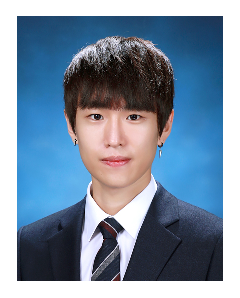
\includegraphics[width=1in,height=1.25in,clip,keepaspectratio]{LSH.eps}}]{Sangheon Lee}
received the B.S. degree in Computer Engineering in 2018 from Sungkyunkwan University, Suwon, Korea. 
He is currently master course student in Department of Electrical and Computer Engineering at Sungkyunkwan University, Suwon, Korea. 
His current research interests include deep-learning, adversarial defense, image classification and natural language processing. 
He is a student member of the IEEE.
\end{IEEEbiography}

\begin{IEEEbiography}[{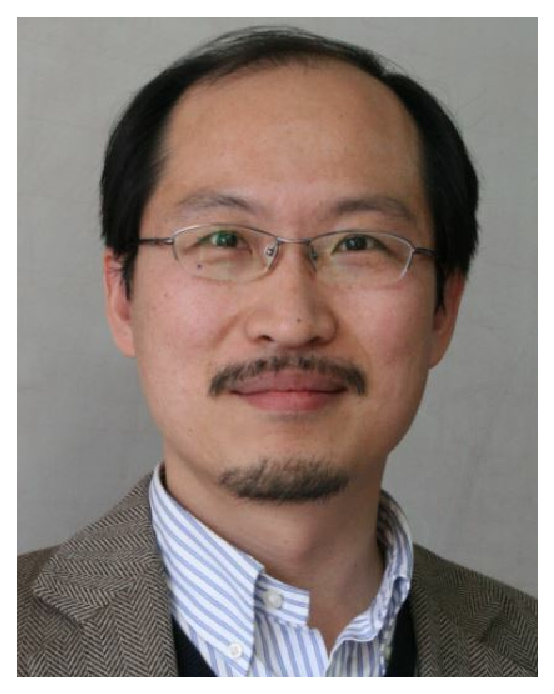
\includegraphics[width=1in,height=1.25in,clip,keepaspectratio]{john.eps}}]{Jee-Hyong Lee}
received his B.S., M.S., and Ph.D. in computer science from Korea Advanced Institute of Science and Technology (KAIST), Daejeon, Rep. of Korea, in 1993, 1995, and 1999, respectively. 
From 2000 to 2002, he was an international fellow at SRI International, USA. 
He is currently working as a professor in the Department of Software at the Sungkyunkwan University, Suwon, Korea. 
His research interests include fuzzy theory and application, intelligent systems, and machine learning. 
He is a fellow member of the IEEE.
\end{IEEEbiography}

\EOD

\end{document}
